\documentclass[10pt]{article}
%\usepackage[margin=1in]{geometry}
\usepackage{amsmath,amssymb,graphicx}
\usepackage{hyperref}
\usepackage{graphicx,float}
\usepackage{mathtools}
\setlength\parindent{0pt}
\usepackage[dvipsnames]{xcolor}

\usepackage{fancyvrb}

% redefine \VerbatimInput
\RecustomVerbatimCommand{\VerbatimInput}{VerbatimInput}%
{fontsize=\footnotesize,
 %
 frame=lines,  % top and bottom rule only
 framesep=2em, % separation between frame and text
 rulecolor=\color{Gray},
 %
 label=\fbox{\color{Black}data.txt},
 labelposition=topline,
 %
 commandchars=\|\(\), % escape character and argument delimiters for
                      % commands within the verbatim
 commentchar=*        % comment character
}



\begin{document}
\title{Assignment 3: Scalar initial value problems}
\author{1212550}
\begin{center}
\section*{Assignment 3: Scalar initial value problems}


The following is a brief report concerning the implementation of a C++ program to solve certain Initial Value Problems.\\
\end{center}

\section{Runge-Kutta methods}

In this assignment we will be considering $\textit{Runge-Kutta}$ (RK) methods to solve the scalar ordinary differential equation
\begin{equation}
    u'(t) = f(u(t),t) \quad u(0) = u_0.
\end{equation}

Let us define $I \coloneqq [t_0,t_0+T]$ and discretise it with $N$ uniform intervals $[t_n,t_{n+1}]$, such that $t_n \coloneqq t_0 + nh$. At each point $t_i$ we let $u_i$ be the approximation of our solution $y(t_i) = y_i$. Moreover we define $f(t_i,u_i) = f_i$. We say that a numerical method is a $\textit{one-step}$ method if they approximate the initial value problem $(1)$ such that $u_{n+1}$ only depends on $u_n$ for all $n \geq 0$. In particular, the RK methods are one-step methods, and we are now in a position to define them.\\

\noindent\fbox{%
    \parbox{\textwidth}{%
        $\textbf{Definition:}$ \textit{Runge-Kutta} methods are one-step methods of the form
\[
u_{n+1} = u_n + hF(t_n,u_n,f,h),
\]
where $F$ is defined as
\begin{align*}
    &F(t_n,u_n,f,h) = \sum_{i=1}^sb_iK_i, \\
    &K_i = f(t_n + c_ih, u_n + h\sum_{j=1}^sa_{ij}K_j), \quad i \in \{1, \dots, s \}.
\end{align*}
The integer $s$ denotes the number of stages of the method.\\
    }
}
\\

Note that the coefficients $A = (a_{ij}) \in \mathbb{R}^{s \times s}$,
$\textbf{b},~ \textbf{c} \in \mathbb{R}^s$ completely determine the RK method. It follows that we can describe the method completely by what is known as its $\textit{Butcher Tableau}$, which are of the form
\begin{center}
\begin{tabular}{ c|c }
 $\textbf{c}$& $A$ \\
  \hline
   & $\textbf{b}^T$  \\
\end{tabular}
\end{center}

\newpage
We will be utilising the following five RK schemes:

\begin{itemize}
    \item Forward Euler (FE): $\quad$
\begin{center}
\begin{tabular}{ c|c }
  0 &    \\
  \hline
    & 1  \\
\end{tabular}
\end{center}

\item Backwards Euler (BE): $\quad$
\begin{center}
\begin{tabular}{ c|c }
  1 & 1   \\
  \hline
    & 1  \\
\end{tabular}
\end{center}

\item Implicit Modpoint (IM):
\begin{center}
\begin{tabular}{ c|c }
  1/2 & 1/2   \\
  \hline
    & 1  \\
\end{tabular}
\end{center}

\item 3 stage Heun (Heun3):
\begin{center}
\begin{tabular}{ c|c c c }
  0 & & &   \\
  1/3 & 1/3 & & \\
  2/3 & 0 & 2/3 &  \\
  \hline
    & 1/4 & 0 & 3/4  \\
\end{tabular}
\end{center}

\item 2 stage DIRK method (DIRK2):
\begin{center}
\begin{tabular}{ c|c c  }
  $\delta$ & $\delta$ &    \\
  $1 - \delta$ & $1 - 2\delta$ & $\delta$  \\
  \hline
    & $1/2$ & $1/2$   \\
\end{tabular}
\end{center}
\end{itemize}

\subsection{Scheme Properties}

\noindent\fbox{%
    \parbox{\textwidth}{%
        \textbf{Definition:} A method is called explicit, if $u_{n+1}$ can be
computed directly in terms of previous values $u_k$, $k < n$. It is called implicit, if $u_{n+1}$ implicitly depends on itself through $f$.
    }
}\\

Note that the schemes will either be explicit or diagonally implicit, with the schemes categorised as follows:
\begin{center}
 \begin{tabular}{||c | c ||}
 \hline
 Explcit & Implicit  \\ [0.5ex]
 \hline\hline
 FE & BE \\
 Heun3 & IM \\
  & DIRK2 \\
 \hline
\end{tabular}
\end{center}
For the implicit cases, we will have to solve the implicit equation,
\[
K_i = f(t + hc_i, u_n + h \sum_{j=1}^{i-1}a_{ij}K_j + ha_{ii}K_i)
\]
in order to run the schemes. Since this equation only depends on previous $K_i$ and itself, we can solve it stage by stage by utilising the \textit{Newton Raphson} method for finding roots.\\

In addition to this, we can use \textbf{Theorem 4.3.9} from the lecture notes to deduce the minimum order of the schemes we are using. They are included in the table below.

\begin{center}
 \begin{tabular}{||c | c ||}
 \hline
 Scheme & Order  \\ [0.5ex]
 \hline\hline
 FE & 1 \\
 BE & 1 \\
 IM & 2 \\
Heun3 & 3 \\
DIRK2 & 2 \\
 \hline
\end{tabular}
\end{center}

\subsection{Implementation}
Equation $(1)$ will be considered for two different right hand functions $f(y,t)$ defined as follows:
\begin{enumerate}
 \item $f(y,t) = 1 - cos(t)(cos(t)-1) - y^2; \quad y_0=0,~T=2\pi$, \\
 with exact solution $y = sin(t)$.

 \item  $f(y,t) = 1 - cos(t)(cos(t)- exp(\lambda t)) - exp(-2\lambda t)y^2 + \lambda y; \quad y_0=0,~T=10,$
 with exact solution $y = exp(-\lambda t)sin(t)$ and $\lambda = -0.1$.
\end{enumerate}

We aim to investigate the convergence rate of the five RK methods for these two test cases, which we will denote as $\textit{Test 1}$ and $\textit{Test 2}$ respectively. To do this we compare the \textit{experimental order of convergence} (eoc) with the theoretical order of convergence. For a series of time steps $(\tau_j)_{j=0}^J$ we define the eoc of the scheme by
\[
eoc_j = \frac{\text{log}(\frac{e_{\tau_j}}{e{\tau_{j-1}}})}{\text{log}(\frac{\tau_j}{\tau_{j-1}})},
\]
where $e_{\tau_j}$ is the discretisation error with the time-step $\tau_j$. \\

For  this  assignment  I  have  implemented  two different header files, \textit{scheme.hh} and \textit{models.hh}. The first file includes a class \textit{DIRK} which defines a general RK method, and speific inhertience classes for the individual shcemes. The class also includes a function \textit{evolve} which updates the approximated solution at each time-step for a given scheme. Included in this function is an implementation of the Newton-Raphson method which is needed for calculating the $K_i$ for implicit schemes. The latter header files includes a structure which defines the models relating to the two right-hand function defined at the beginning of this sub-section.\\

With these files in place, the included $\textit{main.cc}$ file allows the user to input the test, scheme, step-size and number of different time-steps (levels) via the terminal. The program is designed to compute the experimental order of convergence, with added functionality to automatically create data files needed to plot graphs of the error over time. The results from this implementation will be considered in the next section. In addition to this, the maximum error for each time-step and the corresponding eocs are outputted to the terminal.

\section{Testing}

In this section we look at the results of the tests which have been implemented by the C++ program. We first look at the errors.

\subsection{Maximum Error and EOC}
Recall the maximum error is defined to be $e_{\tau_j} = \text{max}_{n=1,...,N}|y_n - u_n|$, such that $N$ is the total number of time-steps and $u_n$ (resp. $y_n$) is the approximated (resp. exact) solution at time-step $n$. The following tables contains the maximum error and the experimental order of convergence for \textit{test 1} and each scheme, for a sequence of time-steps $\{\tau_j\}_{j=0}^{J}$. In particular, we have $\tau_j = \tau_02^{-j}$, $\tau_0 = 0.1$ and $J=12$. Note that in this subsection \textit{the error} will be referring to the maximum error.\\

\textbf{Test 1: FE}
\VerbatimInput{table_1_1.txt}
\textbf{Test 1: BE}
\VerbatimInput{table_1_2.txt}
\textbf{Test 1: IM}
\VerbatimInput{table_1_3.txt}
\textbf{Test 1: Heun3}
\VerbatimInput{table_1_4.txt}
\textbf{Test 1: DIRK2}
\VerbatimInput{table_1_5.txt}

This data seems suggest that the smallest errors occur when we use the Heun3 scheme. Moreover, these errors decrease with each time-step in the sequence $\{\tau_j\}_{j=0}^{J}$ at a fast rate. This aligns with the theory, since Heun3 has the highest theoretical minimum convergence rate. The FE and BE produce very similar results and give the largest errors. This also aligns with the theory, since they have lowest minimum convergence order of all the schemes. DIRK2 produces errors which are much smaller than the IM scheme, although they both have minimum theoretical order 2. Note that this does not go against the theory, since it is the \textit{minimum} order.\\

The error of convergence largely matches the order of the schemes deduced by the theory. Indeed, for the FE and BE schemes we have an eoc which suggest and order of 1. For the IM scheme we have an eoc which suggest an order of 2. There is a slight discrepancy with the Heun3 and DIRK2 schemes. For Heun3, the suggested order from the eoc is higher than the theoretical order for larger time-steps and much lower (even negative) for the last five smallest time-steps. These odd negative results can be attributed to an increase in error as time-steps decrease later on, since in these cases $\text{log}( \frac{e_{\tau_j} }{ e{\tau_{j-1}} }) > 0$ and $\text{log}(\frac{\tau_j}{\tau_{j-1}}) < 0$. The eoc mostly matches the theoretical result for the DIRK2 scheme (for larger time-steps), but again, we get stranger results for smaller time-steps.\\

Next, we analyse the same results for \textit{Test 2} case.\\


\textbf{Test 2: FE}
\VerbatimInput{table_2_1.txt}
\textbf{Test 2: BE}
\VerbatimInput{table_2_2.txt}
\textbf{Test 2: IM}
\VerbatimInput{table_2_3.txt}
\textbf{Test 2: Heun3}
\VerbatimInput{table_2_4.txt}
\textbf{Test 2: DIRK2}
\VerbatimInput{table_2_5.txt}

This data also seems to suggest that the smallest errors occur when we use the Heun3 scheme, closely followed by DIRK2. The IM follows behind these two. FE and BE give the poorest errors. This is all as expected. For the FE scheme, we note that the error is ambiguous for the first four time-steps. This is not too concerning, as we can only guarantee convergence as the time-steps $\tau$ tend towards zero. As the time-steps get smaller, the FE and BE schemes give similar errors.

The eoc varies more widely for Test 2. Due to the errors \textit{inf} found in the table for FE, the first four eoc values are unstable also. Afterwards, they seems to match the expected order. Although the eoc for BE seems inconsistent with the theory for larger time-steps, it is roughly 1 as expected for smaller time-steps. The IM scheme gives an eoc which is roughly 2 for most time-steps as expected. It is hard to see an average for the eoc values in the tables for Heun3 and DIRK2 due to large fluctuations.

\subsection{Plots}

For a given time-step $\tau$, we will now be considering the error between the approximate solution $u_n$ and the exact solution $y_n$ at each of the discretisation points $t_n = t_0 + n\tau $ for $n=1, \dots , N$, which we defined at the beginning of section 1. We may write this error succinctly as $e_n = |u_n-y_n|$ for $n = 1,\dots,n$. It follows that $e_\tau = \text{max}_{n=1,\dots,N}e_n$. Note that in this subsection, for a given $n$, \textit{the error} will be referring to $e_n$. \\

Below are graphs which plot the error for Test 1 and 2 over time, for time-step sizes $\tau = 0.1$ and $\tau = 0.01$. Note that for Test 1 (resp. Test 2) we will be running over the interval $[0,2\pi]$ (resp. $[0,T]$). For the first test, the graphs have been plotted for all of the schemes. For Test 2, the graphs have been plotted for all schemes apart from FE, due to the instability we encountered in the previous subsection. For readability, the y-axis (which describes the error) is set in log-scale for readability. For each scheme, the maximum error which we considered in subsection 2.1 will correspond to the global maximum of it's respective graph.

 \begin{figure}[H]
 \begin{center}
    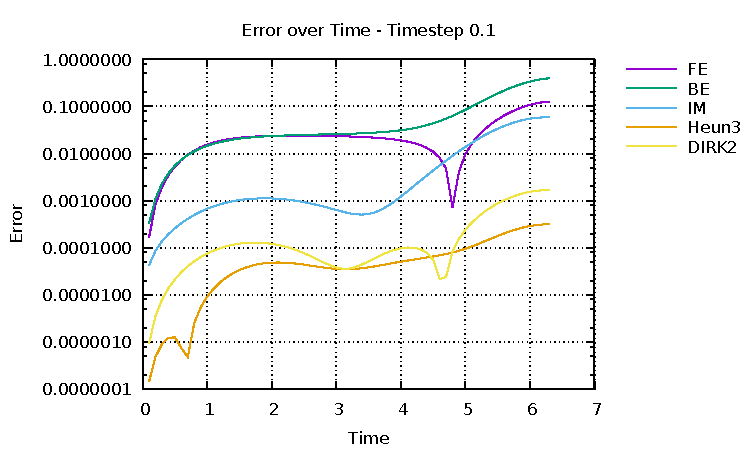
\includegraphics[width=1\textwidth]{plot1_01.pdf}
  \end{center}
  \caption{Test 1: time-step $\tau = 0.1$.
  \label{fig: 1_01}}
\end{figure}

 \begin{figure}[H]
 \begin{center}
    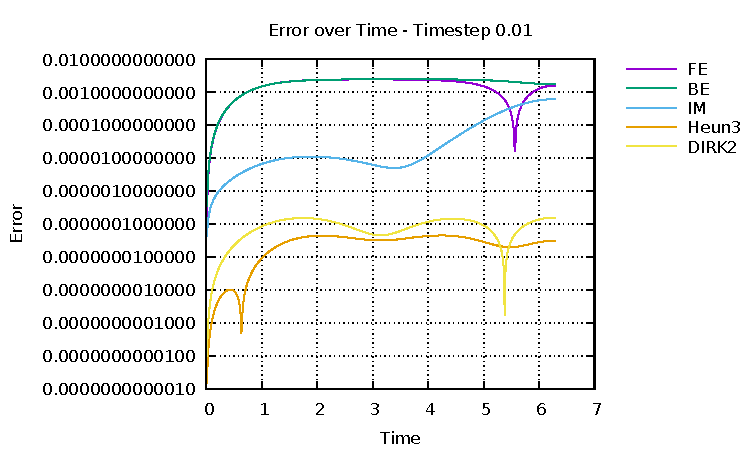
\includegraphics[width=1\textwidth]{plot1_001.pdf}
  \end{center}
  \caption{Test 1 : time-step $\tau = 0.01$.
  \label{fig: 1_001}}
\end{figure}

 \begin{figure}[H]
 \begin{center}
    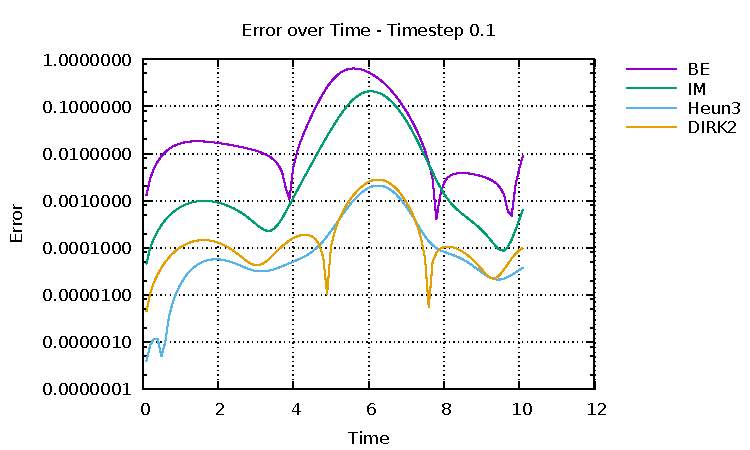
\includegraphics[width=1\textwidth]{plot2_01.pdf}
  \end{center}
  \caption{Test 2: time-step $\tau = 0.1$.
  \label{fig:2_01}}
\end{figure}

 \begin{figure}[H]
 \begin{center}
    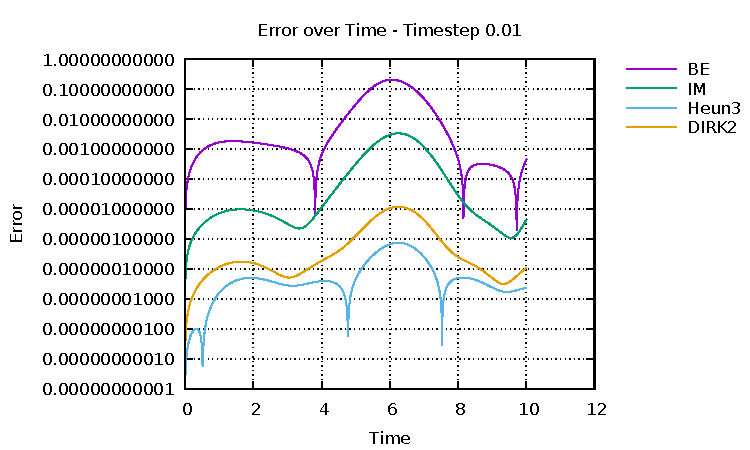
\includegraphics[width=1\textwidth]{plot2_001.pdf}
  \end{center}
  \caption{Test 2: time-step $\tau = 0.01$.
  \label{fig: 2_001}}
\end{figure}

\subsection{The Number of Evaluations}

We now look at how many times we need to evaluate $f$ and $df$ during the course of running the C++ code for each scheme. We do this by implementing a counter which increases by 1 at each evaluation. This total is outputted to the terminal for each time-step in the sequence $\{\tau_j \}_{j=0}^{12}$, which we defined earlier. By comparing the counters, we can conjecture which scheme is the most efficient. Noting that the general pattern is the same from any chosen time-step, I have only included a table for the counter of each scheme (for Test 1 and Test 2) for $\tau = 0.1$. These results can be seen below.


\begin{center}

    \begin{tabular}{|c||c|c|c|c|c|}
    \hline
      $\tau = 0.1$  & FE & BE & IM & Heun3 & DIRK2\\
    \hline
       \hline
       Counter for Test 1  & 63 & 382 & 378& 189 & 1004   \\
       \hline
       Counter for Test 2  & 101  & 674& 606 & 303 & 1650  \\
        \hline
    \end{tabular}
\end{center}

For both tests, the FE scheme seems to be the most efficient. Indeed, the schemes FE and Heun3 are more efficient than the rest, due to the fact that they are explicit (the implicit schemes need numerous evaluations of $f$ and $df$ due to the Newton-Raphson implementation). We note that DIRK2 is the seems to be the least efficient scheme, although it has a better theoretical order than FE. I would conjecture that Heun3 is the best scheme to choose for implementation since the data suggest it has the best order of all of the schemes and, except for FE, is the most efficient scheme.
\end{document}
